\documentclass[11pt]{article}
\usepackage{geometry}                % See geometry.pdf to learn the layout options. There are lots.
\geometry{a4paper}                   % ... or a4paper or a5paper or ... 
%\usepackage[parfill]{parskip}    % Activate to begin paragraphs with an empty line rather than an indent
\usepackage{graphicx}
\usepackage{amssymb}
\usepackage{epstopdf}
\usepackage{tikz} % allows for figures
\usepackage{float} % allows [H] on figure definition
\usepackage{wrapfig}
\usepackage{amsmath} % allows for matrix

\DeclareGraphicsRule{.tif}{png}{.png}{`convert #1 `dirname #1`/`basename #1 .tif`.png}



\graphicspath{ {images/} }

% user macros
\newcommand{\Z}{\mathbb{Z}}
\newcommand{\R}{\mathbb{R}}
\newcommand{\C}{\mathbb{C}}
% end user macros

\title{A Space of Circle Packing Algorithms}
\author{
  Kevin Pratt\\
  \texttt{kevin.pratt@uconn.edu}
  \and
  Connor Riley\\
  \texttt{connor.riley@uconn.edu}
    \and
  Donald R. Sheehy\\
  \texttt{don.r.sheehy@uconn.edu}
}\date{March 2016}
\begin{document}
\maketitle

\section{Introduction}
The Circle Packing Theorem provides a wonderful link between questions of geometry, topology, combinatorics and complex analysis. Discovered by Paul Koebe and later reintroduced by William Thurston, Circle Packings have become a principle area of study for many mathematicians and geometers. While the formal definition will be introduced later, the intuition for Circle Packings must be developed. A Circle Packing is a configuration of circles with a specified pattern of tangencies \cite{stephenson05introduction}. The Circle Packings most often studied are those that require the interior of the circles to be disjoint, called unilevant packings, this means the circles are non-overlapping \cite{stephenson05introduction}. In this case, a Circle Packing can be thought of as a graph formed by a set of circles which have no overlapping interiors, where each circle kisses its surrounding circles. Two circles kiss or osculate when they intersect at exactly one point. 

\begin{wrapfigure}{r}{0.4\textwidth}
  \begin{center}
    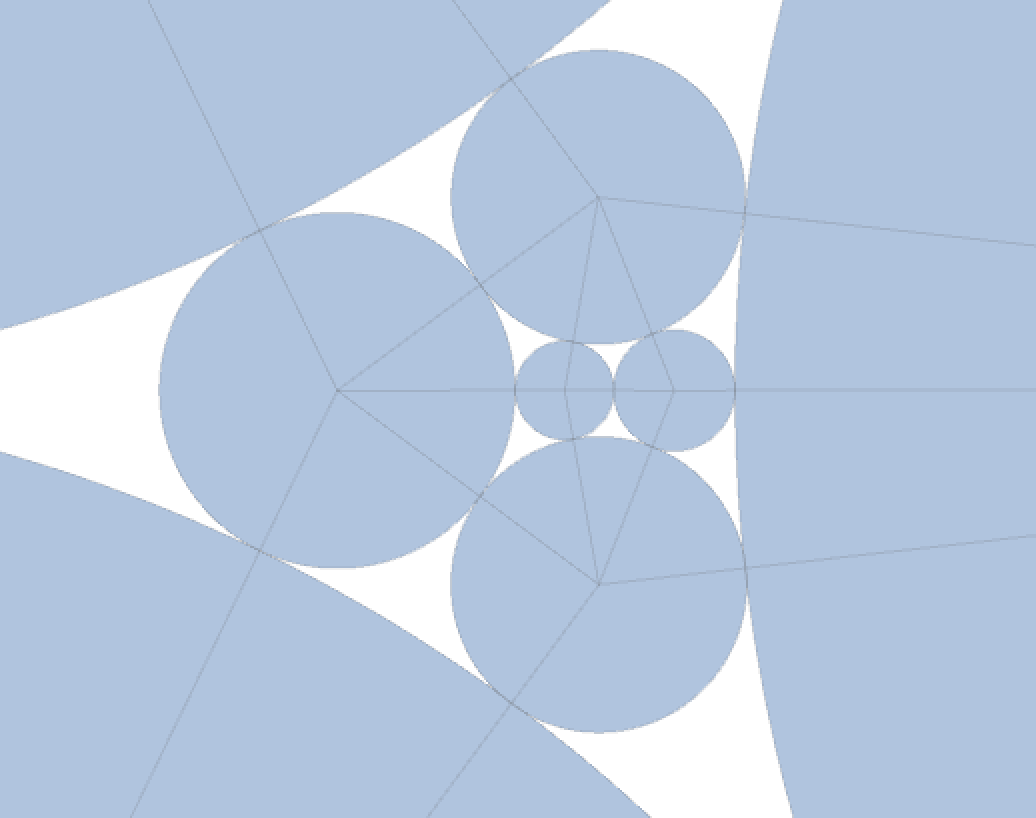
\includegraphics[scale=.18,width=0.45\textwidth]{circlepacking_1}
  \end{center}
  \caption{A unilevant circle packing in a triangle.}
\end{wrapfigure}

Common geometric settings for circle packing are the $euclidean$ $plane$, $the$ $sphere$ and the $hyperbolic$ $plane$. Each pair of circles in a packing forms a tangent pair, and the empty space between each $triple$ forms a $interstice$ \cite{stephenson05introduction}. A $flower$ is the next level of structure, which consists of a central circle and some number of $petal$ circles. The number of petals defines the $degree$ of the central circle. Every circle in a packing has to have a flower, this is called the $local$ $planarity$ condition \cite{stephenson05introduction}. Note that while not all circle packings are unilevant, the ones discussed in this paper and created by the corresponding application will all be unilevant. This means that the interior of all the circles will be mutually disjoint and that the angle sum at each label will be $2\pi$.

The objective of this paper is to explore the space of Circle Packing Algorithms. To accomplish this goal the theory of Circle Packings will be explored. The other goal is to introduce the reader to the world of Circle Packings, and to do this, basic Geometric principles must be introduced. If you, the reader, are familiar with geometry, then we encourage you to skip the following section.

\section{Introduction to Geometric Figures}
\subsection{Graphs}
A \textbf{graph} is an ordered pair $G=(V,E)$ which represents a set of objects where some of these objects are linked. In the denotation $G=(V,E)$, $V$ stands for the vertices or objects, and $E$ stands for the edges or links. Edges in a graph can be directed or undirected, however, we will focus on undirected edges in our application.

  A component or \textbf{connected component} of a graph is a subgraph in which any two vertices are connected to each other by a path which is connected to no additional vertices in the supergraph.

  A \textbf{loop} is when a vertex has an edge connecting it to itself.
  
  A graph with multiple edges is one which has two or more edges connect the same two vertices.

  A graph is \textbf{connected} when there is a path between every pair of vertices \cite{mathworld:ConnectedGraphs}. 
  In a connected graph every vertex is reachable. A graph with just one vertex is connected. A graph is said to be \textbf{k-connected} if there does not exist a set of k-1 vertices whose removal disconnects the graph. Typically we will work with 3-connected graphs - this means that three vertices would have to be removed to disconnect the graph.
  
  A \textbf{simple graph} is an unweighted, undirected graph, containing no loops or multiple edges \cite{mathworld:SimpleGraphs}. 
  A simple graph may either be connected or disconnected.
  
  A \textbf{planar graph} is one that can be embedded in the plane. 
  In other words, the graph can be drawn on the plane in such a way that its edges intersect only at their endpoints (no edges cross each other) \cite{mathworld:PlanarGraph}.
  
  A graph $G' = (V',E')$ is a \textbf{subgraph} of $G$ ($G' \subseteq G$), if $V' \subseteq V$ and $E' \subseteq E$. Two important types of subgraphs are:
  \begin{itemize}
  \item A $path$ between two vertices $v_1$ and $v_k$ in $G$ is a subgraph $G' \subseteq G$ with $V' = \{v_1,...v_k\}$ and 
  $E' 	= \{\{v_1,v_2\},...\{v_{k-1}, v_k\}\}$. We write $G' = G_{v_1}^{v_k}$.
  \item A $k-cycle$ in $G$ is a subgraph $G'\subseteq G$ with $V' = \{v_1,...,v_k\}$ and 
  $E' = \\ \{\{v_1,v_2\},...\{v_{k-1}, v_k\}, \{v_k,_1\}\}$
  \item A $Y-Graph$ in $G$ that connects $v_1,v_2, v_3 \in V$ is a subgraph $G' \subseteq G$ such that there exists a vertex $w \in V \backslash \{v_1,v_2, v_3\}$ and paths $G_{v_1}^w, G_{v_2}^w, G_{v_3}^w$ that are disjoint except for the common endpoint $w$.
  \end{itemize}
  
Now that we have established the some basic geometric concepts, we can introduce the formal definition of a circle packing.

\section{Circle Packings}
If $\xi$ is an oriented surface with a distance metric then a collection $P = \{c_v\}$ of circles in $\xi$ is said to be a circle packing for a complex $K$ if (1) $P$ has a circle $c_v$ associated with each vertex $v$ of $K$, (2) two circles $c_u$, $c_v$ are tangent whenever $<u,v>$ is an edge of $K$, and (3) three circles $c_u$, $c_v$, $c_w$ form a positively oriented triple in $\xi$ whenever $<u,v,w>$ forms a positively oriented face of $K$ \cite{stephenson05introduction}. 

Technically, circle packings exists for any planar graph, however it is often simpler algorithmically to work with 3-connected, triangulated planar graphs. If we limit our study to these types of graphs, then every circle packing on these graphs is a Weighted Delaunay Triangulation. 

\subsection{Delaunay Triangulations}
	A \textbf{triangulation}, also referred to as a \textbf{maximal planar graph}, is a planar graph in which there is no way to add another edge and have the graph continue to be planar \cite{meshGeneration}. In practice, this means that each face is bounded by three edges - each face is a triangle. This is explained by $Whitney's$ $Theorem$ which concludes that if a graph is planar and 3-connected, all the faces of the graph will be the same shape.

Formally, a triangulation of $S$, a finite set of points in the plane, is a simplicial complex $\tau$ such that $S$ is the set of vertices in $\tau$, and the union of all the simplices in $\tau$ is the convex hull of $S$ \cite{meshGeneration}. Where a simplex is the generalization of the notion of a triangle to arbitrary dimensions.

There are many specific types of triangulations in mathematics, however, we will focus on Delaunay and Weighted Delaunay triangulations.

To explain Delaunay triangulations, some properties of triangles must first be defined. The \textbf{circumcircle} of a triangle is the circle which passes through all three of its vertices \cite{mathworld:Circumcenter}. The center of the circumcircle is called the \textbf{circumcenter} and the radius is the \textbf{circumradius}. The circumcenter can be found by finding the intersection of the \textbf{altitudes}, which are formed by drawing a perpendicular line from each vertex to the opposite side of the triangle.
  
A \textbf{Delaunay Triangulation} for a set of points $P$ is the triangulation of those points such that no point in $P$ is inside the circumcircle of any other triangle \cite{meshGeneration}. Delaunay triangulations are important largely because in two dimensions they maximize the minimum angle in the triangulation.

\subsubsection{The Edge Flip Algorithm}
An alternate way of describing a Delaunay triangulation is one in which every edge in the triangulation is $locally$ $Delaunay$ \cite{meshGeneration}. For an edge $e$ in the triangulation $\tau$, if $e$ is an edge of fewer than two triangles, then it is automatically locally Delaunay. If $e$ is an edge of exactly two triangles, then $e$ is locally Delaunay if it has an open circumcirlce containing no vertex of either triangle. 

As a result of this property, a trivial algorithm can be formulated that creates a Delaunay triangulation. If $S$ is the point set, this algorithm begins with any triangulation $\tau$ of $S$. Begin with a list of all the edges in the triangulation. Remove an edge from the list, check if the edge is still in the triangulation and if so, if it is locally Delaunay. If the edge is present but not locally Delaunay, flip the edge and add the four surrounding edges to the list of edges to check. This yields an $O(n + k)$ runtime, where in the worst case $k = O(n^2)$ \cite{meshGeneration}.

This leaves one issue, how do we determine whether an edge is locally Delaunay or not. This can be done using the $InCircle$ $test$. Given triangle $abc$ and point $p \in P$ $InCircle(a,b,c,d) \neq 1$ if $abc$ if Delaunay. 
	\begin{equation}
		InCircle(a,b,c,d) = \frac{sign(det
		\begin{bmatrix}
    			a & b & c & d \\
    			\|a\|^2 & \|b\|^2 & \|c\|^2 & \|d\|^2 \\
    			1 & 1 & 1 & 1 \\
		\end{bmatrix} 
		)}{ccw(a,c,b)}
	\end{equation}
	\begin{equation}
		ccw(a,c,b) = det[c-a,b-a] = det
		\begin{bmatrix}
    			a & b & c \\
    			1 & 1 & 1\\
		\end{bmatrix} 
	\end{equation}
This equation is simply asking if point $d$ is above of below the plane defined by points $a,b,c$. This is because for any point $a = (x,y)$ the parabolic lifting is defined as $h(x,y) = x^2 + y^2 = \| 
	\begin{bmatrix} 
		x \\
		y \\ 
	\end{bmatrix} 
	\|^2$.
	As a result for any point $a$ the parabolic lifting of $a$, $a'$ is equal to $
	\begin{bmatrix} 
		a \\ 
		\| a \|^2 \\ 
	\end{bmatrix}$. 
	Therefore the lifting of all three points is equal to
	$\begin{bmatrix}
    			a & b & c \\
    			\|a\|^2 & \|b\|^2 & \|c\|^2 \\
	\end{bmatrix}$ 
	is the parabolic lifting of the points $a,b,c$.

An incremental Delaunay algorithm can now be constructed. Given a Delaunay triangulation and a point $p$ to add to the set of points $P$, a new Delaunay triangulation can be created containing point $p$ by first finding the triangle containing point $p$ and then splitting the triangle three ways. This is done by creating edges from point $p$ to each vertex of the triangle. Now that a we have a triangulation the edge flip algorithm is run to make it a Delaunay triangulation. The base case of this algorithm is when you only have three points, in which case, you simply connect the points to create a triangle. 

Given a finite point set $S$ the parabolic lifting transforms the Delaunay triangulation of $S$ into faces of a convex polyhedron in three dimensions. This property makes it easy to accept that every finite point set has a Delaunay triangulation because every finite point set has a polyhedral convex hull. In turn, this means that every finite point set has a Circle Packing.

\subsubsection{Voronoi Diagrams}
Delaunay triangulations are the geometric $dual$ of Voronoi diagrams. A \textbf{Voronoi diagram} is the partitioning of a plane into regions based on distance to points in a specific subset of the plane. Formally, the Voronoi diagram of metric space $X$ with a distance function $d$, where $K$ is the set of indices and $P_k, k \in K$ is a tuple of nonempty subsets in the space $X$, is composed of Voronoi cells $C_k$ associated with the site $P_k$. $C_k$ is the set of all points in $X$ whose distance to $P_k$ is not greater than their distance to the other sites $P_j$ \cite{voronoiDiagrams}. 

While Voronoi diagrams can be understood without understanding geometric duals, expanding our understanding of duals will help build the intuition for the connection between the Voronoi diagram and the Delaunay triangulation. This means that the faces, also called 2-cells, of the Voronoi diagram correspond to the points of the Delaunay triangulation. The edges of the Voronoi diagram, also called 1-cells, correspond to the edges, 0-cells, of the Delaunay triangulation and the vertices of the Voronoi diagram correspond to faces of the Delaunay triangulation. The edges of the Voronoi Diagram are orthogonal to the edges of the Delaunay triangulation. These relationships are a result of the fundamental relationships between a dual and primal graph.

In two dimensions, those relationships are as follows: point $p = 
	\begin{bmatrix}
		p_x \\
		p_y \\
	\end{bmatrix} \leftrightarrow $ line $p* = 
	\begin{bmatrix}
		2p_x \\
		-p_y \\
	\end{bmatrix}$ and line $\ell = 
	\begin{bmatrix}
		\ell_n \\
		\ell_b \\
	\end{bmatrix}$ point $\ell* = 
	\begin{bmatrix}
		\frac{1}{2}\ell_n
		-\ell_b
	\end{bmatrix}$. In three dimensions, the relationships undergo similar transformations $point \leftrightarrow plane$, $line \leftrightarrow line$. As a result, lifting the points of a graph from the plane to a 3-dimensional space then taking the dual of those points to obtain hyperplanes and lastly, projecting those planes back onto the original 2-dimensional plane yields a Voronoi diagram and as a result is another way to obtain the Delaunay triangulation.
	
Lastly, just as the Delaunay triangulation is the lower hull of the parabolic lifting, the Voronoi diagram is the upper hull.

\subsubsection{Weighted Delaunay Triangulations}

In the triangulation the weighted disks assigned to the vertices to find the orthocenter end up being the circles in the packing and the orthocircle becomes the inscribed circle of the triangle. 

The \textbf{orthocircle} is the circle that is orthogonal to the disks around the vertices of a triangle. The radii of these disks represent the weight of each vertex of the triangle. If these disks have radii equal to zero, then the orthocircle is equal to the circumcircle.

\section{Misc.}


\bibliographystyle{plain}
\bibliography{references}
\end{document}  